\documentclass[12pt]{article}
\usepackage{graphicx}
\usepackage{wrapfig}
\usepackage{subcaption}
\begin{document}
\graphicspath{d:/LATEX courses}
\begin{figure}[t]
\begin{minipage}{0.6\linewidth}
\vspace{5cm}
\hspace{0cm}
Eiffel Tower was constructed from  1887 to 1889 as the entrance to thev1889 World's Fair and was initually criticised by some of France's leading artist and initellectuals for its design, but it has become a global cul-tural icon of France and one of the most recognisable structures in the world.[3].The Eiffel Tower is the most visited momment with an entrance fee in the world;6.91  million people ascended it in 2015.\\ \\
\end{minipage}
\begin{minipage}{0.5\linewidth}
\vspace{0cm}
\hspace{0cm}
\centering
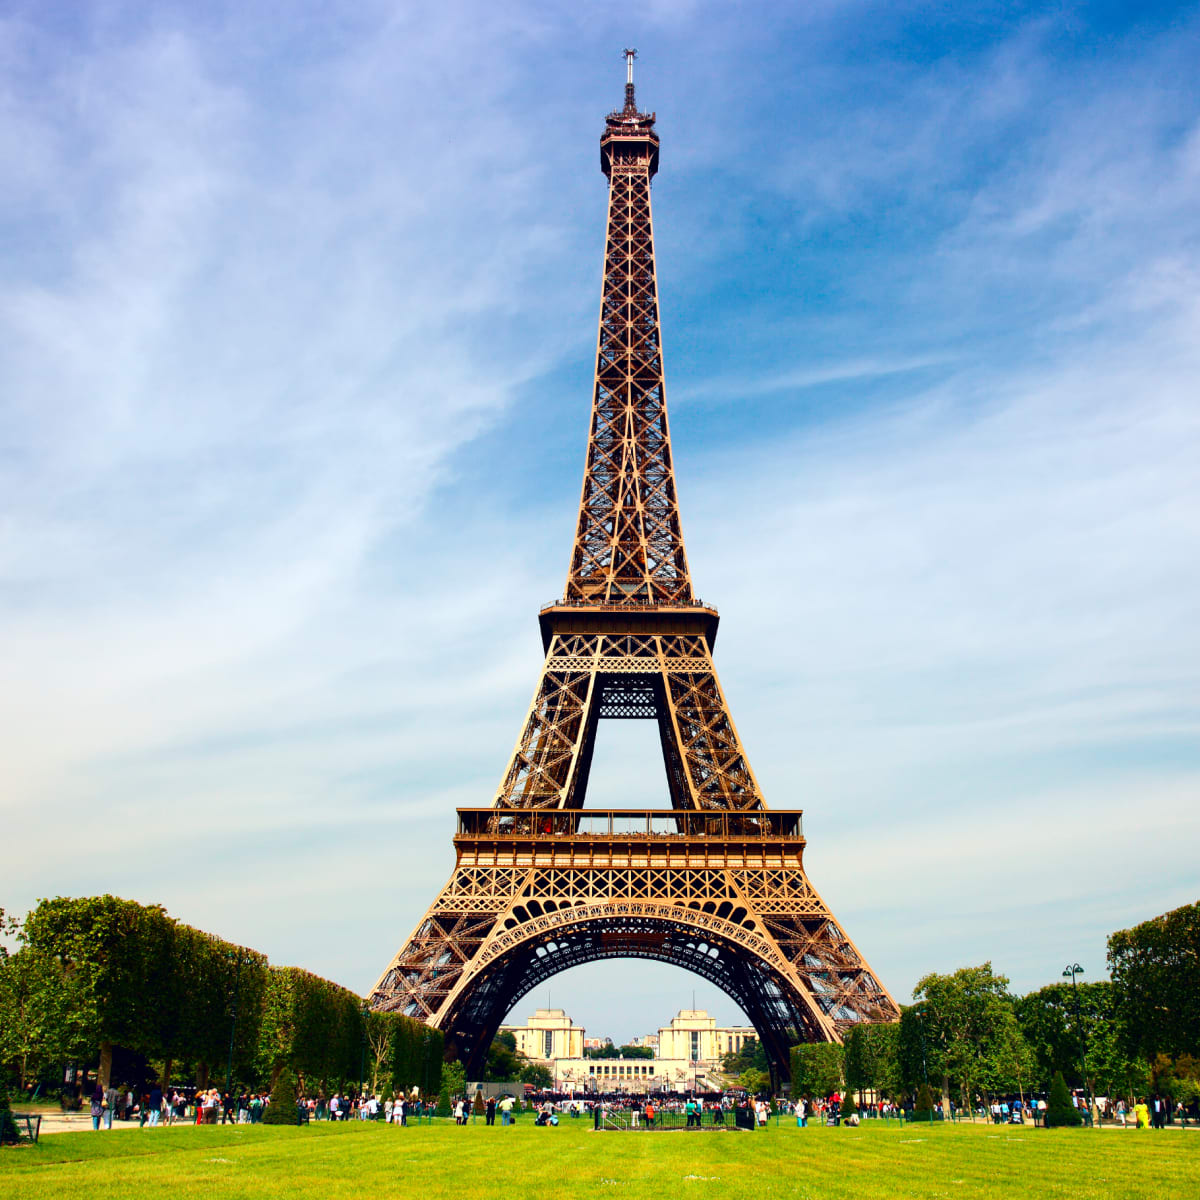
\includegraphics[width=5cm,height=4cm]{paris}
\caption{The Eif-\\fel Tower}
\vspace{-5.1cm}
\hspace{-2cm}
\end{minipage}
\begin{minipage}{1\linewidth}
The tower is 324 meters (1,063 ft) tall, about the same height as an 81 - storey building, and the tallest structure in Paris. Its base is square, measuring 125 metres (410 ft) on each side.During its constructure , the Eiffel Tower surpassed the Washington Monument to become the tallest man -made structure in the world,a title it held for 41 years until the Chrysler Building in New York City was finished in 1930.
\end{minipage}
\end{figure}
\end{document}
